\documentclass{../paper}

\newcommand{\eq}[1]{Eq.~\eqref{#1}}
\newcommand{\eqs}[2]{Eqs.~\eqref{#1}--\eqref{#2}}
\newcommand{\fig}[1]{Fig.~\ref{#1}}

\begin{document}

\title{Testing Bell's inequality with entangled photons}

\author{Iago B.~Mendes\,\orcidlink{0009-0007-9845-8448}}
\email{ibrazmen@oberlin.edu}
\affiliation{Department of Physics and Astronomy, Oberlin College, Oberlin, Ohio 44074, USA}

\date{\today}

\begin{abstract}
  Bell's inequality, $|S| \leq 2$, must hold true for any hidden local variable theory. In this experiment, we performed a test of quantum mechanics by evaluating this inequality with polarization-entangled photon pairs generated through spontaneous parametric down-conversion in a nonlinear birefringent crystal. An analysis of our prepared state revealed a deviation from the ideal maximally entangled state, with the polarization angle $\theta_l$ estimated at approximately $25\deg$, rather than the expected $45\deg$. Consequently, our measured value of $S = 1.8(1)$ fails to violate Bell's inequality. A ``corrected'' model assuming ideal entanglement predicts $S = 2.0(1)$, but the high uncertainty prevents a definitive conclusion. Despite this, the experiment provided valuable hands-on experience with foundational tests of quantum mechanics. Future work would benefit from better preparation of the state and increased data collection time to reduce statistical noise.
\end{abstract}

\maketitle

\section{Introduction}

The field of quantum optics, which explores the quantum nature of light and its interaction with matter, has its roots in the early 20th century with the development of quantum mechanics itself. While light had been successfully described as an electromagnetic wave by Maxwell's theory, phenomena such as the photoelectric effect and blackbody radiation needed a quantized description, in which light is composed of discrete packets of energy called photons \cite{Einstein1905}. This revolutionary idea, introduced by Albert Einstein, laid the foundation for understanding the fundamental quantum properties of light.

Another pivotal moment in the development of quantum optics was the theoretical work of John Bell addressing a long-standing debate about the completeness of quantum mechanics \cite{Bell1964}, sparked by the Einstein-Podolsky-Rosen (EPR) paradox \cite{Einstein1935}. EPR argued that quantum mechanics might be an incomplete theory because it seemed to allow for ``spooky action at a distance'', where measurements on one entangled particle instantaneously affect the state of another, regardless of the distance separating them. EPR then proposed the existence of ``local hidden variables'' that would predetermine the outcomes of measurements. Bell's work showed that any local hidden variable theory must satisfy a statistical inequality, which is violated in quantum mechanics. This provided an experimentally testable way to distinguish between quantum mechanics and local hidden variable theories.

The first experimental test of Bell's inequality was done by Clauser, Horne, Shimony, and Holt (CHSH) \cite{Clauser1969}, which provided evidence against local hidden variable theories and supported the predictions of quantum mechanics. Subsequent experiments solidified these findings \cite{Aspect1982, Weihs1998}, having improved precision and addressing potential loopholes.

In this experiment, we use a pair of entangled photons, generated by a nonlinear birefringent crystal, to test Bell's inequality. In Section \ref{sec:theory}, we provide an overview of the CHSH form of Bell's inequality. Section \ref{sec:methods} describes the experimental setup and methods used to generate and measure the photon pairs. In Section \ref{sec:results}, we present the results of our measurements, including an analysis of the prepared state and an evaluation of Bell's inequality. Finally, we conclude in Section \ref{sec:conclusion} with a summary of our findings and possible areas of improvement.

\section{Theory}\label{sec:theory}

We use non-linear optic properties of birefringent crystals to generate entangled photon pairs, which are then sent to a couple of detectors that are preceded by polarizers. If $\alpha$ and $\beta$ represent the angles from the detector polarizers to the vertical, it can be shown that the probability that both detections come out as ``vertical'' is given by
\begin{equation}\label{eq:Pvv}
  \begin{aligned}
    P_{VV}(\alpha, \beta)
    &= \sin^2\alpha \sin^2\beta \cos^2\theta_l \\
    &\quad + \cos^2\alpha \cos^2\beta \sin^2\theta_l \\
    &\quad + \frac{1}{4} \sin2\alpha \sin2\beta \sin2\theta_l \cos\phi_m
  \end{aligned}
\end{equation}
\cite{Dehlinger2002}, where $\theta_l$ represents the initial polarization of the laser beam and $\phi_m$ is an averaged accumulated phase shift.

In the maximally entangled state ($\theta_l = 45\deg$ and $\phi = 0\deg$), \eq{eq:Pvv} reduces to
\begin{equation}\label{eq:Pvv-QM}
  P^\text{QM}_{VV}(\alpha, \beta) = \frac{1}{2} \cos^2(\beta - \alpha)
\end{equation}
\cite{Dehlinger2002}. However, if we consider a local realistic hidden variable theory (HVT), it can be shown that such maximally entangled state would lead to a probability of
\begin{equation}\label{eq:Pvv-HVT}
  P^\text{HVT}_{VV}(\alpha, \beta) = \frac{1}{2} - \frac{|\beta - \alpha|}{\pi}
\end{equation}
\cite{Dehlinger2002}.

In studying the feasibility of a HVT, John Bell derived an inequality that must be true for any HVT \cite{Bell1964}. In the context of \eq{eq:Pvv-HVT}, it was found in \cite{Clauser1969} that this inequality can be expressed as
\begin{equation}\label{eq:Bell-inequality}
  |S| \leq 2
\end{equation}
\cite{Dehlinger2002}, where
\begin{align}
  S &\equiv E(a,b) - E(a,b') + E(a',b) + E(a',b') \label{eq:S} \\
  E(\alpha,\beta) &\equiv P_{VV}(\alpha,\beta) + P_{VV}(\alpha_\perp,\beta_\perp) \label{eq:E-inP} \\
                  &\notag \qquad\qquad\quad - P_{VV}(\alpha,\beta_\perp) - P_{VV}(\alpha_\perp,\beta),
\end{align}
and the angles $a$, $b$, $a'$, and $b'$ are defined as in \fig{fig:angles}.

\begin{figure}
  \centering
  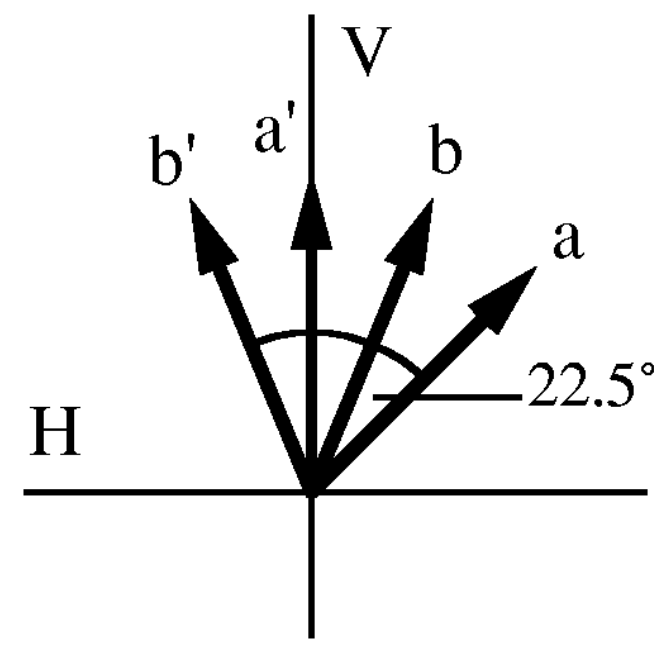
\includegraphics[width=0.6\columnwidth]{assets/angles.png}
  \caption{Schematic showing the angles used in \eq{eq:S}. Here, $a = -45\deg$, $b = -22.5\deg$, $a = 0\deg$, and $b' = 22.5\deg$. This figure is reproduced from \cite{Dehlinger2002}.}
  \label{fig:angles}
\end{figure}

This means that if a HVT exists, then \eq{eq:Bell-inequality} must be satisfied. However, if the quantum mechanical prediction from \eq{eq:Pvv-QM} is correct, then the value of $S$ will be greater than 2, violating \eq{eq:Bell-inequality}.

It is important to note that Quantum Mechanics does not necessarily violate \eq{eq:Bell-inequality} in all cases. However, we have chosen the angles in \fig{fig:angles} such that the quantum mechanical prediction for $S$ is maximized (and greater than 2) in the maximally entangled state \cite{Dehlinger2002}, thus violating \eq{eq:Bell-inequality}.

\section{Methods}\label{sec:methods}

Our experimental setup is shown in \fig{fig:setup}. A vertically polarized 407 nm laser beam is sent into a couple of wave plates. The half-wave plate (HWP) is used to rotate the polarization of the photons to be as close as possible to the desired angle $\theta_l = 45\deg$, while the quarter-wave plate (QWP) corrects the phase shift from the crystal so that $\phi_m \approx 0$. We will discuss how we have calibrated the angles of these wave plates in the next section. If done correctly, the photons emerging from these wave plates will be in the maximally entangled state,
\begin{equation}\label{eq:entangled-state}
  \frac{1}{\sqrt{2}} (\ket{HH} + \ket{VV})
\end{equation}
\cite{LabManual}, where $\ket{H}$ and $\ket{V}$ represent states of photons polarized horizontally and vertically, respectively. If not done correctly, the photons will not be in the maximally entangled state, and the value of $S$ might not be help us in evaluating Bell's inequality.

\begin{figure}
  \centering
  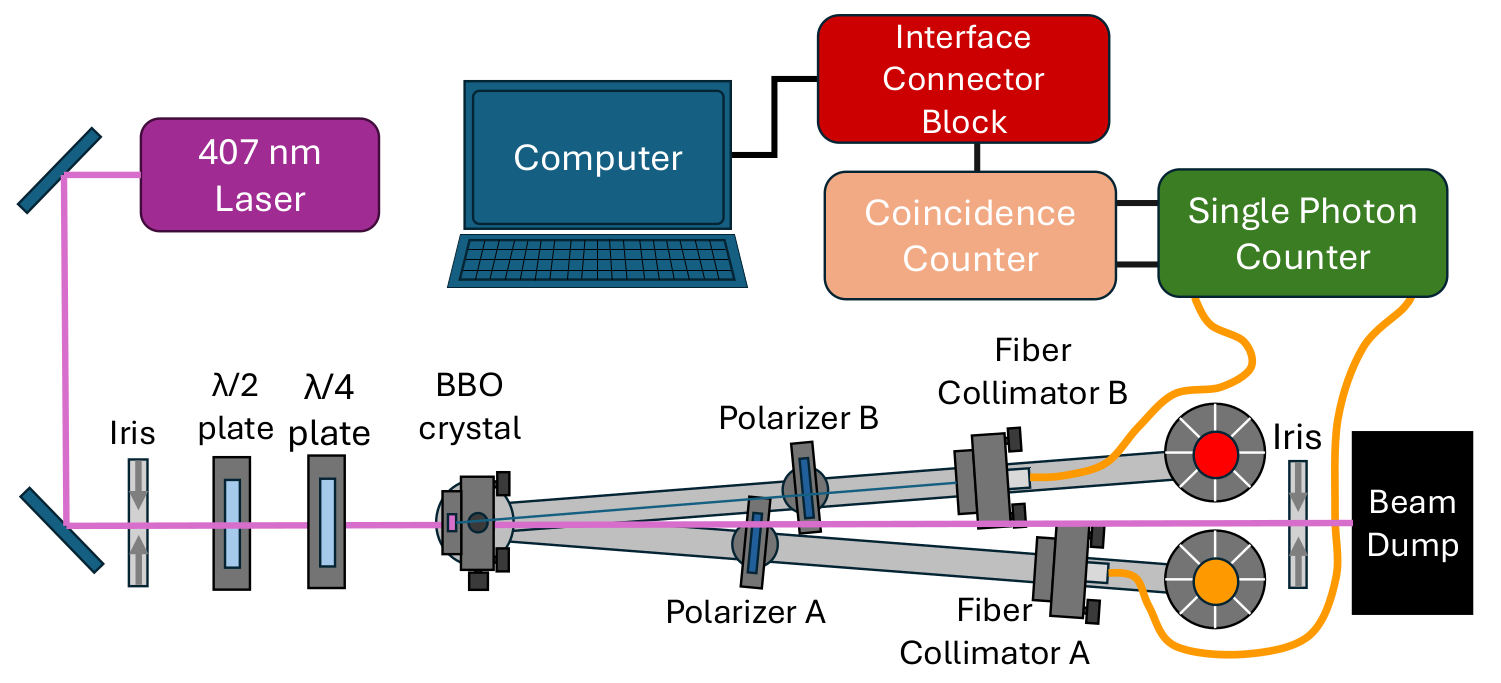
\includegraphics[width=1.0\columnwidth]{assets/setup.png}
  \caption{Experimental setup. This figure is reproduced from \cite{LabManual}.}
  \label{fig:setup}
\end{figure}

The entangled photons are then sent to a pair of beta barium borate (BBO) crystals, where they undergo spontaneous parametric down-conversion, producing two orthogonally polarized beams \cite{Dehlinger2002}. This conversion is represented in \fig{fig:photon-conversion}. The angles $\theta$ and $\alpha$ are related to the laser frequency $\omega_p$ by
\begin{equation}\label{eq:photon-conversion}
  \frac{\sin^2\theta}{\tilde n_e(\omega_p)^2} + \frac{\cos^2\theta}{n_o(\omega_p)^2} = \frac{\sec^2\theta}{n_o(\frac12\omega_p)^2}
\end{equation}
\cite{LabManual}, where $\tilde n_e$ and $n_o$ are the extraordinary and ordinary refractive indices of the BBO crystal, respectively. For our BBO crystal, these refractive indices are specified by
\begin{align}
  n_o(\lambda)^2 &= 2.7359 + \frac{0.01878}{\lambda^2 - 0.01822} - 0.01354 \lambda^2, \label{eq:ordinary-index} \\
  \tilde n_e(\lambda)^2 &= 2.3753 + \frac{0.01224}{\lambda^2 - 0.01667} - 0.01515 \lambda^2 \label{eq:extraordinary-index}
\end{align}
\cite{LabManual}, where $\lambda$ is the wavelength measured in microns. Knowing that our BBO crystal was cut so that its optic axis is $\theta = 30\deg$, we can use \eqs{eq:photon-conversion}{eq:extraordinary-index} to find $\alpha \approx 3.21\deg$. This angle tells us how to orient the polarizers relative to the BBO crystal so that we can detect the two converted beams. It is essential to check this in the alignment process.

\begin{figure}
  \centering
  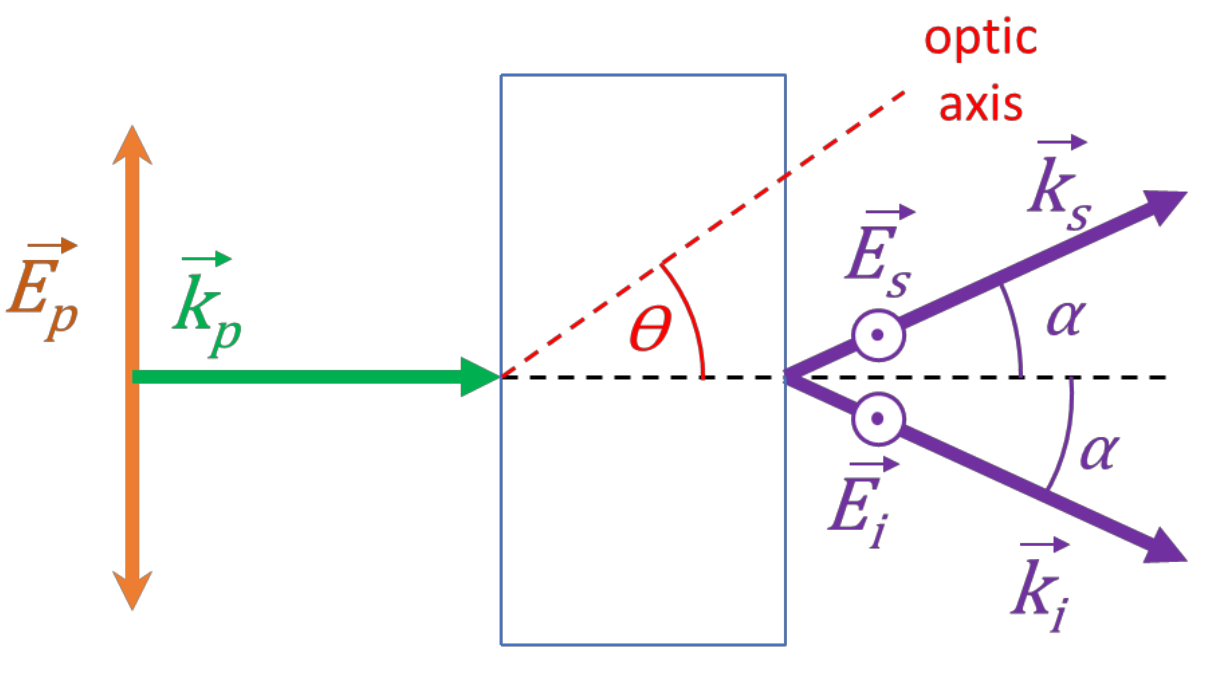
\includegraphics[width=0.9\columnwidth]{assets/photon-conversion.png}
  \caption{Representation of the photon conversion in the BBO crystal. This figure is reproduced from \cite{LabManual}.}
  \label{fig:photon-conversion}
\end{figure}

The two beams are then sent to polarizers at angles $\alpha$ and $\beta$ from the vertical. The photons are then detected by a couple of single-photon detectors. The detectors are connected to a coincidence counter, which records the number of times both detectors detect a photon at the same time in a coincidence window of $\tau = 25$ ns \cite{LabManual}.

The coincidence counter gives us $N(\alpha,\beta)$, the number of coincidences for a given configuration of the polarizers. We can re-write \eq{eq:E-inP} in terms of $N(\alpha,\beta)$ as
\begin{equation}\label{eq:E}
  \footnotesize
  \begin{aligned}
    E(\alpha,\beta) \equiv \frac{N(\alpha,\beta) + N(\alpha_\perp,\beta_\perp) - N(\alpha,\beta_\perp) - N(\alpha_\perp,\beta)}{N(\alpha,\beta) + N(\alpha_\perp,\beta_\perp) + N(\alpha,\beta_\perp) + N(\alpha_\perp,\beta)}
  \end{aligned}
\end{equation}
\cite{Dehlinger2002}. With this, we can calculate the value of $S$ using \eq{eq:S}.

It's important to note that we need to subtract background single-photon counts from our measurements. By blocking the beam path, we measured the background single-photon count rate in detector A $\dot N_A^\text{background} \approx 923$ Hz and in detector B $\dot N_B^\text{background} \approx 624$ Hz. After measuring the raw counts in both detectors ($N_A^\text{raw}$ and $N_B^\text{raw}$), we define
\begin{align}
  N_A &\equiv N_A^\text{raw} - T \dot N_A^\text{background}, \\
  N_B &\equiv N_B^\text{raw} - T \dot N_B^\text{background},
\end{align}
where $T$ is the duration of the measurement.

Additionally, we know from \cite{LabManual} that there is an expected number of accidental coincidences given by
\begin{equation}
  N^\text{ac} = N_A N_B \frac{\tau}{T}.
\end{equation}
After measuring the raw coincidences $N^\text{raw}$, we can then define the corrected coincidences as
\begin{equation}
  N \equiv N^\text{raw} - N^\text{ac}.
\end{equation}

\section{Results}\label{sec:results}

Our first set of measurements (shown in Table \ref{tab:5-measurements}) was taken with $T=60$ s in order to analyze our prepared state. Our second set of measurements (shown in Table \ref{tab:16-measurements}) was taken with $T=8$ minutes to be used in to evaluate $S$.

This section is divided into three parts. First, we look at the calibration of the wave plates, which is essential to prepare the photons in the maximally entangled state. Then, we analyze the state of the photons we have been able to create. Finally, we calculate the value of $S$ in an attempt to evaluate Bell's inequality.

\begin{table}
  \centering
  \begin{tabular}{cc|ccc|c}
    $\alpha$ & $\beta$   & $N_A^\text{raw}$ & $N_B^\text{raw}$ & $N^\text{raw}$ & $N$  \\
    \hline
    $0\deg$  & $0\deg$   & $66195$          & $64087$	         & $10$           & $10$ \\
    $90\deg$ & $90\deg$  & $76322$          & $97093$	         & $17$           & $17$ \\
    $0\deg$  & $90\deg$  & $64369$          & $96829$	         & $4$            & $4$  \\
    $45\deg$ & $45\deg$  & $74406$          & $86618$	         & $19$           & $19$ \\
    $45\deg$ & $-45\deg$ & $73555$          & $76268$	         & $6$            & $6$  \\
  \end{tabular}
  \caption{Set of 5 measurements taken with $T = 60$ s.}
  \label{tab:5-measurements}
\end{table}

\begin{table}
  \centering
  \begin{tabular}{cc|ccc|c}
    $\alpha$  & $\beta$    & $N_A^\text{raw}$ & $N_B^\text{raw}$ & $N^\text{raw}$ & $N$   \\
    \hline
    $-45\deg$ & $-22.5\deg$ & $548510$         & $565065$         & $76$          & $75$  \\
    $-45\deg$ & $22.5\deg$  & $546175$         & $626254$         & $24$          & $23$  \\
    $-45\deg$ & $67.5\deg$  & $546660$         & $807829$         & $63$          & $61$  \\
    $-45\deg$ & $112.5\deg$ & $545895$         & $738278$         & $120$         & $118$ \\
    $0\deg$   & $-22.5\deg$ & $522904$         & $522904$         & $48$          & $48$  \\
    $0\deg$   & $22.5\deg$  & $520821$         & $625289$         & $37$          & $36$  \\
    $0\deg$   & $67.5\deg$  & $519373$         & $808650$         & $27$          & $26$  \\
    $0\deg$   & $112.5\deg$ & $522048$         & $744202$         & $19$          & $18$  \\
    $45\deg$  & $-22.5\deg$ & $605777$         & $578021$         & $41$          & $40$  \\
    $45\deg$  & $22.5\deg$  & $597014$         & $632914$         & $75$          & $73$  \\
    $45\deg$  & $67.5\deg$  & $592238$         & $810973$         & $141$         & $138$ \\
    $45\deg$  & $112.5\deg$ & $593777$         & $745974$         & $66$          & $64$  \\
    $90\deg$  & $-22.5\deg$ & $623314$         & $568441$         & $39$          & $38$  \\
    $90\deg$  & $22.5\deg$  & $617312$         & $620594$         & $45$          & $43$  \\
    $90\deg$  & $67.5\deg$  & $619769$         & $817720$         & $175$         & $172$ \\
    $90\deg$  & $112.5\deg$ & $621931$         & $746304$         & $139$         & $136$ \\
  \end{tabular}
  \caption{Set of 16 measurements taken with $T = 8$ minutes.}
  \label{tab:16-measurements}
\end{table}

\subsection{Calibration of wave plates}

To calibrate the HWP, we varied its angle from the vertical $\lambda_H$ and recorded $N(\alpha, \beta)$ in two configurations: $(\alpha,\beta) = (0\deg, 0\deg)$ and $(\alpha,\beta) = (90\deg, 90\deg)$. We then fitted the data to the expected shape of $\sin^2(\lambda_\text{HWP})$ using {\tt SciPy}'s {\tt curve\_fit} procedure \cite{SciPy}. The results are shown in the left panel of \fig{fig:wave-plates}. Seeking the state in \eq{eq:entangled-state}, we want to equalize $N(0\deg,0\deg)$ and $N(90\deg,90\deg)$, which is satisfied when $\lambda_H \approx 62\deg$.

We calibrated the QWP similarly. We varied its angle from the vertical $\lambda_Q$ and recorded $N(45\deg,45\deg)$, which we want to maximize. The resulting data and fit are shown in the right panel of \fig{fig:wave-plates}. From this, we see that the maximum of $N(45\deg,45\deg)$ is satisfied when $\lambda_Q \approx 140\deg$.

All of these measurements had a duration of $T = 30$ s.

\begin{figure*}
  \centering
  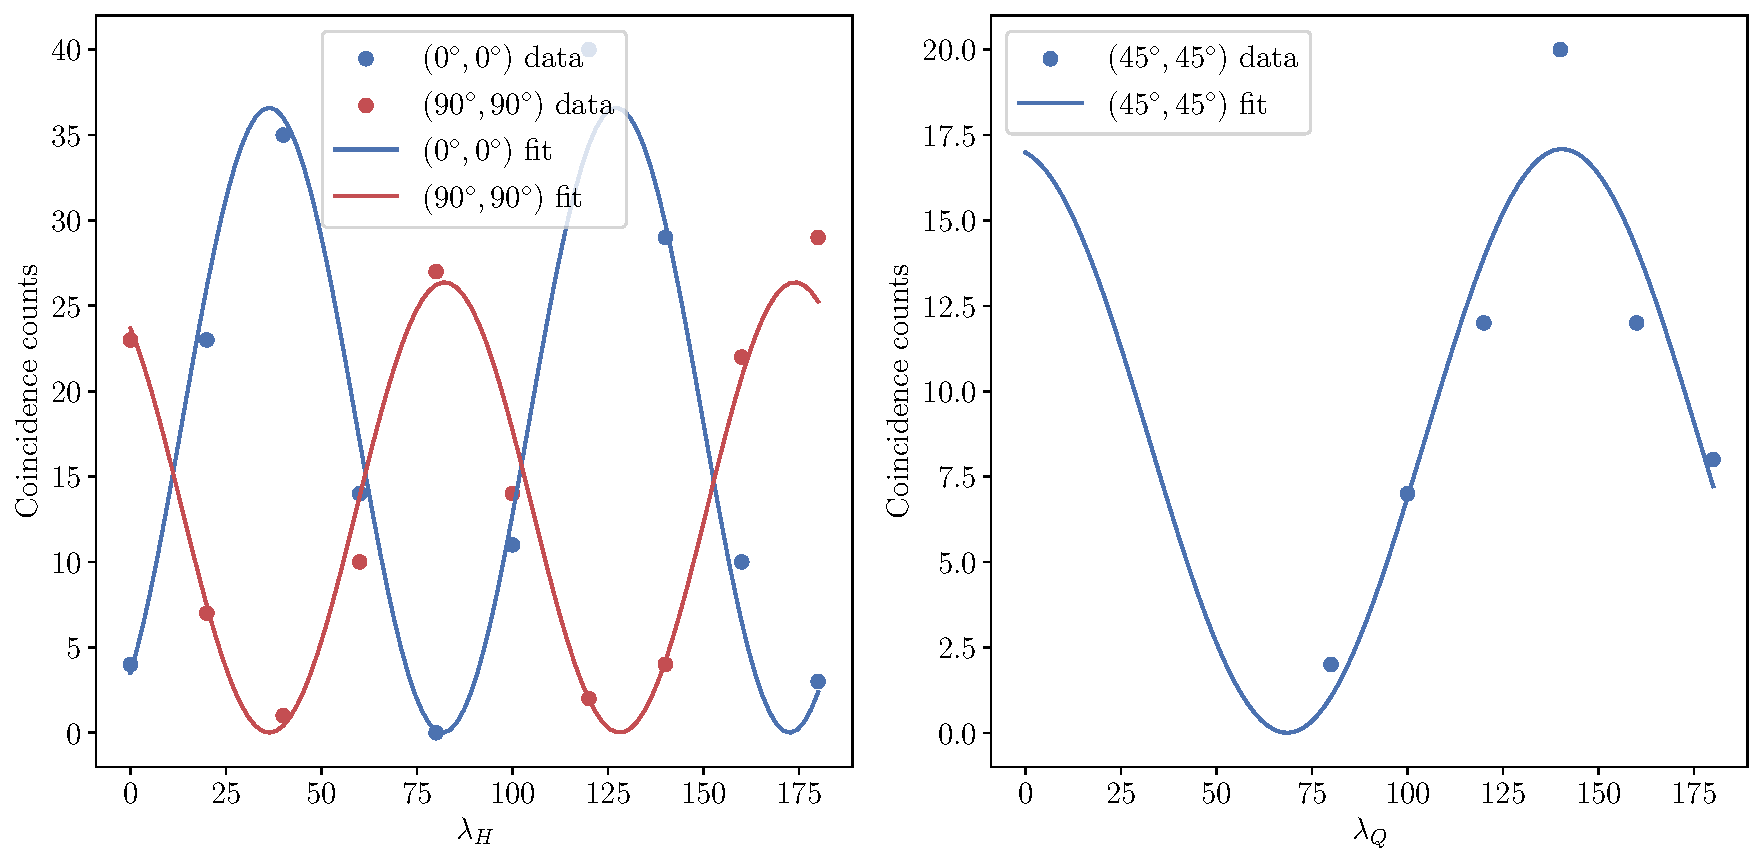
\includegraphics[width=0.7\textwidth]{analysis/wave-plates.pdf}
  \caption{Calibration of the HWP (left) and the QWP (right).}
  \label{fig:wave-plates}
\end{figure*}

\subsection{Analysis of state}

From \cite{LabManual}, we know that the expected number of coincidences can be modelled by
\begin{equation}\label{eq:N-model}
  \begin{aligned}
    N(\alpha,\beta)
    &= A (\sin^2\alpha \sin^2\beta \cos^2\theta_l \\
    &\qquad + \cos^2\alpha \cos^2\beta \sin^2\theta_l \\
    &\qquad + \frac{1}{4} \sin2\alpha \sin2\beta \sin2\theta_l \cos\phi_m) + C
  \end{aligned}
\end{equation}
and that the model parameters can be estimated with
\begin{align}
  C &= N(0\deg, 90\deg), \label{eq:model-C} \\
  A &= N(0\deg, 0\deg) + N(90\deg, 90\deg) - 2 C, \label{eq:model-A} \\
  \tan^2\theta_l &= \frac{N(90\deg,90\deg) - C}{N(0\deg,0\deg) - C}, \label{eq:theta_l} \\
  \cos\phi_m &= \frac{1}{\sin 2\theta_l} \left( 4 \frac{N(45\deg, 45\deg) - C}{A} - 1 \right) \label{eq:model-phi_m}.
\end{align}

Using the results from Table \ref{tab:5-measurements}, we can use the analytical expressions in \eqs{eq:model-C}{eq:model-phi_m} as a quick check of the state we have prepared. Doing so, we obtain
\begin{align}
  A &= 19(6), \label{eq:estimate1-A} \\
  \theta_l &= 55(8)\deg, \label{eq:estimate1-theta_l} \\
  \cos\phi_m &= 2(1), \label{eq:estimate1-phi_m} \\
  C &= 4(2). \label{eq:estimate1-C} 
\end{align}
\eq{eq:estimate1-theta_l} clearly deviates from the desired $\theta_l = 45\deg$, which is likely due to improper calibration of the wave plates or misalignment of the other optical components. Additionally, note that we should have $|\cos\phi_m| \leq 1$, but this is violated by \eq{eq:estimate1-phi_m}. This suggests that \eqs{eq:model-C}{eq:model-phi_m} might not be the proper way to describe our prepared state. A comparison between the measurements from Table \ref{tab:5-measurements} and the model with the analytic check parameters in \eqs{eq:estimate1-A}{eq:estimate1-C} is shown in \fig{fig:state}(a).

In order to get a better estimate of the prepared state used in the data of actual interest, we can fit the measurements from Table \ref{tab:16-measurements} into a model like \eq{eq:N-model}. We performed such fit using {\tt SciPy}'s {\tt least\_squares} procedure \cite{SciPy}. This fit gives us
\begin{align}
  A &= 200(20), \label{eq:estimate2-A} \\
  \theta_l &= 25(4)\deg, \label{eq:estimate2-theta_l} \\
  \phi_m &= -0.003\deg \pm 300000\deg, \label{eq:estimate2-phi_m} \\
  C &= 20(7) \label{eq:estimate2-C}
\end{align}
Unfortunately, \eq{eq:estimate2-theta_l} is again far from the desired $\theta_l = 45\deg$. Also, note that the high error in \eq{eq:estimate2-phi_m} indicates that the least squares fit did not see any changes in the numerical residuals when varying $\phi_m$. A comparison between the measurements from Table \ref{tab:16-measurements} and the model with the fit parameters in \eqs{eq:estimate2-A}{eq:estimate2-C} is shown in \fig{fig:state}(b).

The significant difference between \eq{eq:estimate1-theta_l} and \eq{eq:estimate2-theta_l} is concerning and should be further investigated in future experiments. One possible source for this discrepancy is in how the two approaches handle the difficulty in estimating $\phi_m$, leading to the strange results in \eq{eq:estimate1-phi_m} and \eq{eq:estimate2-phi_m}.

\begin{figure*}
  \centering
  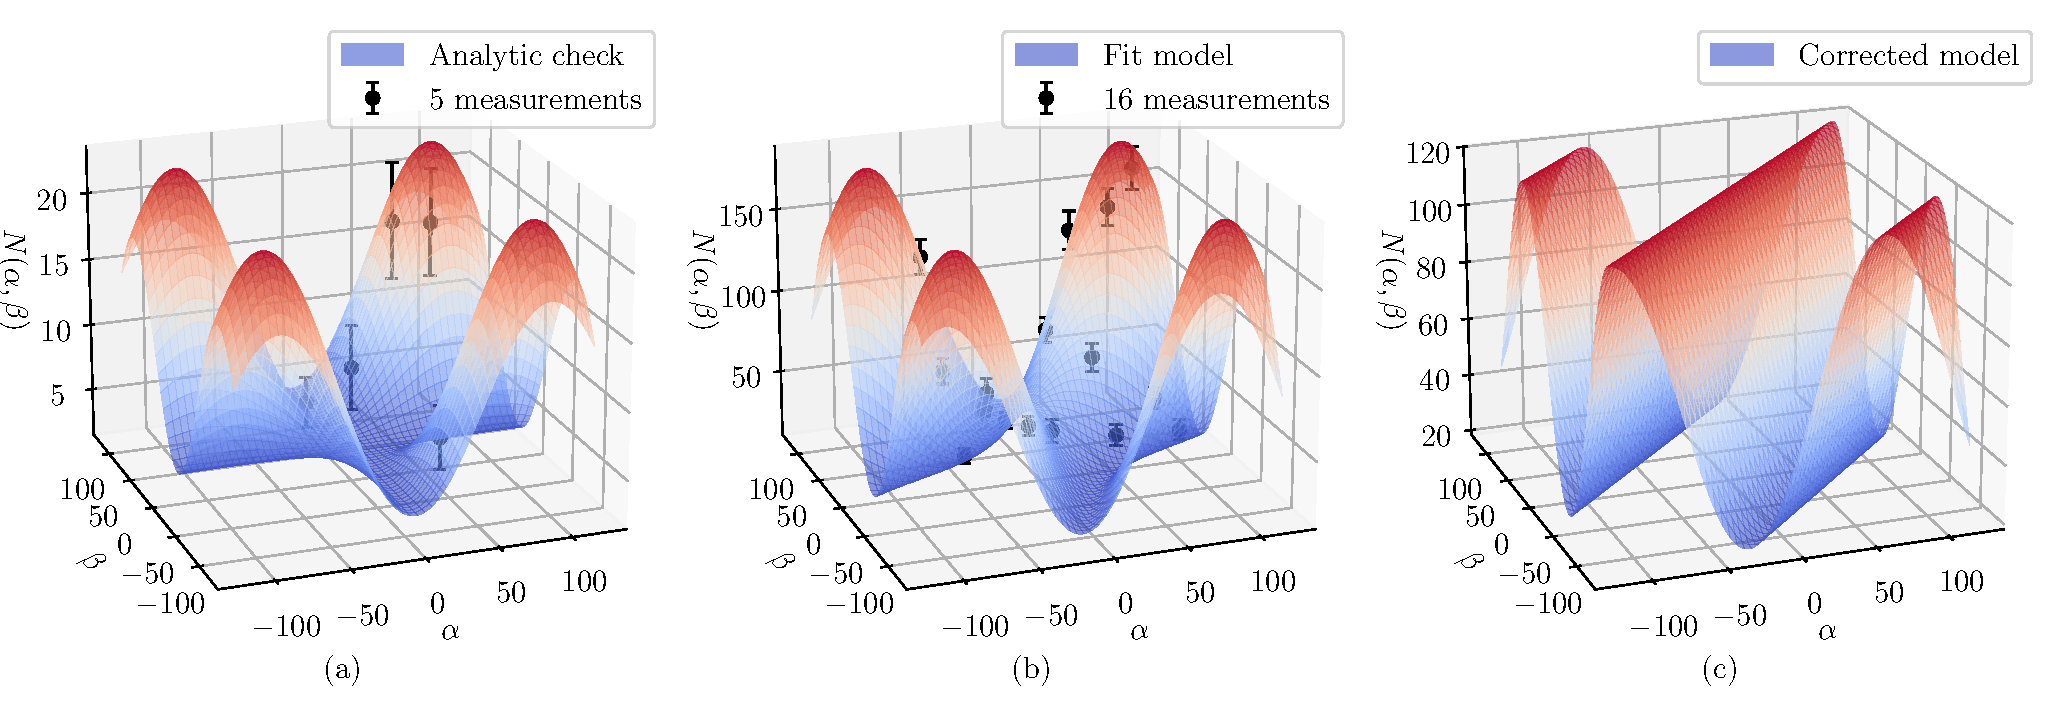
\includegraphics[width=0.95\textwidth]{analysis/state.pdf}
  \caption{Visualizations of $N(\alpha,\beta)$ based on the model in \eq{eq:N-model}. (a) uses the analytic parameters from \eqs{eq:estimate1-A}{eq:estimate1-C}. (b) uses the fit parameters from \eqs{eq:estimate2-A}{eq:estimate2-C}. (c) uses the fit parameters from \eqs{eq:estimate2-A}{eq:estimate2-C} but enforces $\theta_l = 45\deg$.}
  \label{fig:state}
\end{figure*}

\subsection{Bell's inequality}

Using the measurements in Table \ref{tab:16-measurements}, we can calculate the value of $S$ using \eq{eq:S} and \eq{eq:E}. The resulting value is
\begin{equation}
  S = 1.8(1).
\end{equation}
Unfortunately, we do not get the expected violation of Bell's inequality, as this value is less than 2. This is likely due to the fact that we did not properly prepare the photons in the maximally entangled state, as discussed in the previous section.

That said, we can try to estimate what $S$ would be if we use our model from \eq{eq:N-model} with the parameters found in \eqs{eq:estimate2-A}{eq:estimate2-C}, except that we enforce $\theta_l = 45\deg$. The result of this ``corrected'' model is shown in \fig{fig:state}(c). The contrast between \fig{fig:state}(b) and \fig{fig:state}(c) highlights that our state's value of $\theta_l$ has a significant impact in the distribution of our coincidence measurements. With this, we can re-calculate $S$ using \eq{eq:S} and \eq{eq:E} to find
\begin{equation}
  S = 2.0(1).
\end{equation}
While this brings us closer to the expected violation of Bell's inequality, it is still not enough to conclude that we have violated \eq{eq:Bell-inequality} because of our uncertainty.

\section{Conclusion}\label{sec:conclusion}

Using polarization-entangled photon pairs generated through spontaneous parametric down-conversion in a birefringent crystal, we conducted an experiment to test Bell's inequality. Our analysis of the prepared state revealed deviations from the ideal maximally entangled state, as indicated by the estimated value of $\theta_l \approx 25\deg$, which differs significantly from the desired $\theta_l = 45\deg$. Therefore, the calculated value of $S = 1.8(1)$ did not show a violation of the Bell inequality ($|S| \leq 2$). This non-ideal entangled state preparation is likely due to imperfect calibration of the wave plates or misalignment in the optical setup. While a ``corrected'' model assuming a maximally entangled state ($\theta_l = 45\deg$) gave us a value of $S = 2.0(1)$, the high uncertainty still prevents a definitive conclusion regarding the violation of Bell's inequality. That being said, this experiment provided a great opportunity to gain hands-on experience with quantum optics and the details of testing fundamental aspects of quantum mechanics.

Future work should focus on refining the preparation of the maximally entangled state. This could involve a more precise calibration of the half-wave and quarter-wave plates, as well as a thorough re-alignment of the entire optical path. It is also essential to investigate the discrepancy observed in the estimated $\theta_l$ between the analytical expressions in \eqs{eq:model-C}{eq:model-phi_m} and the fit according to the model in \eq{eq:N-model}. Furthermore, increasing the data acquisition time for each measurement point could reduce statistical uncertainties and provide a more robust evaluation of $S$.

\begin{acknowledgements}
  This work was done in collaboration with Anya Molodtsova under the supervision of Professor Yumi Ijiri.
\end{acknowledgements}

\bibliography{refs}

\end{document}
